
%%%%%%%%%%%%%%%%%%%%%%%%%%%%%%%%%%%%%%%%%%%%%%%%%%%%%%%%%%%%%%%%%%%%%%%%%%%%%%
%%%%%%%%%%%%%%%%%%%%%%%%%%%%%%%%%%%%%%%%%%%%%%%%%%%%%%%%%%%%%%%%%%%%%%%%%%%%%% 

%\subsection{Proof for arbitrary $n \geq 7$}
%\label{subsec: proof for n greater-equal than 7}

In this sub-section we prove that Condition~{\MixCond} in Theorem~\ref{thm: miscibility characterization}(a)
is sufficient for perfect mixability when $n\geq 7$. 
Let $C$ be a configuration that satisfies Condition~{\MixCond},
where  $C\cup \braced{\mu} \ingroundset \integers$ and $\nofdroplets{C} = n$.  
Also, let the factorization of $n$ be $n = 2^{\tau_0}p_1^{\tau_1} p_2^{\tau_2} ... p_s^{\tau_s}$, 
where $\braced{p_1,p_2,...,p_s} = \barp$ is the set of 
the odd prime factors of $n$ and $\braced{\tau_1,\tau_2,...,\tau_s}$ are their corresponding multiplicities.

If $A\ingroundset\integers$ is a configuration with $\nofdroplets{A} = n$ 
(where $n$ is as above) and $\average(A)\in\integers$, 
we will say that $A$ is \emph{$\barp$-incongruent} if $A$ is $p_r$-incongruent for all $r$.
If $A$ is $\barp$-incongruent then, by Lemma~\ref{lem: uniform wrt coprime numbers}(a),
it is $b$-incongruent for all $b$ that are powers of $p_r$'s, which,
by Corollary~\ref{cor: mc prime power factors}, implies that $A$ satisfies Condition~{\MixCond}.
Further, if $A$ is also not near-final
then Lemma~\ref{lem: mixability m = 2} implies that $\nofconcentrations{A}\ge 3$.
We summarize these observations below. (They will be often used in this section
without an explicit reference.)

\begin{observation}%-------------
	\label{obs: A mod-nouniform properties}
	Assume that a configuration $A\ingroundset \integers$ with $\average(A)\in\integers$ is $\barp$-incongruent.
	Then
	\textrm{(a)} $A$ satisfies Condition~{\MixCond}, and
	\textrm{(b)} if $A$ is not near-final then $\nofconcentrations{A}\ge 3$.
\end{observation}%---------------

%%%%%%%%%%%%%%%%%%%%

\myparagraph{Proof outline}
The outline of the sufficiency proof for $n\ge 7$ is as follows (see Figure~\ref{fig: proof outline n >= 7}):
Assume that $C$ is not perfectly mixed.
Instead of dealing with $C$ directly,
we will consider a $\barp$-incongruent configuration $\intermC\ingroundset\integers$ with $\intermmu = \average(\intermC)\in\integers$
that is ``equivalent'' to $C$ in the sense
that $C$ is perfectly mixable with precision at most $1$ if and only if $\intermC$ is perfectly mixable
with precision $0$. 

It is thus sufficient to show that $\intermC$ is perfectly mixable with precision $0$.
To this end, we first apply some mixing operations to $\intermC$, producing only integer concentrations,
that convert $\intermC$ into a configuration $E$ such that:
%
\begin{description}
	\item{(I.0)} $E\ingroundset \integers$ and $\average(E) = \intermmu$,
	\item{(I.1)} $E$ has at least $2$ distinct non-singletons, and
	\item{(I.2)} $E$ is $\barp$-incongruent.
\end{description}

We refer to the three conditions above as Invariant~(I).
Then we show that any configuration $E$ that satisfies Invariant~(I)
has a pair of different concentrations whose mixing either preserves Invariant~(I)
or converts $E$ into a near-final configuration.
We can thus repeatedly mix such pairs, preserving Invariant~(I), until 
we produce a near-final configuration, that, by the previous section,
can be perfectly mixed with precision $0$. 

\begin{figure}[ht]
	\begin{center}
		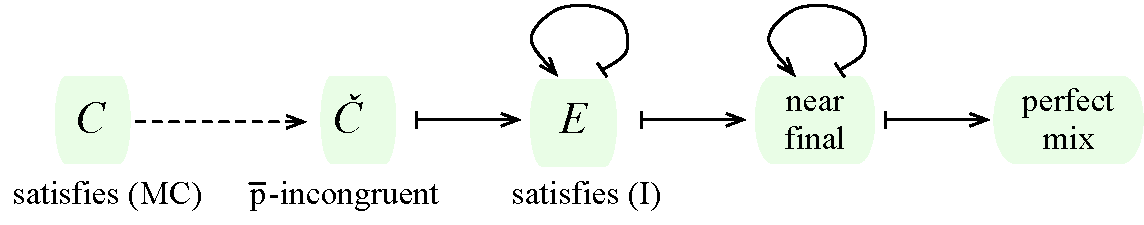
\includegraphics[width = 4.2in]{proof_outline_n_ge_7.pdf}
		\caption{Proof outline for $n\ge 7$. The first dashed arrow represents
			replacing $C$ by $\intermC$. Solid arrows represent mixing operations.}
		\label{fig: proof outline n >= 7}
	\end{center}
\end{figure}

%%%%%%%%%%%%%%%%%%%%

\myparagraph{Replacing $C$ by $\intermC$}
We now explain how to modify $C$. We will do it in steps.
First, let $C' = C-c_1$, for some arbitrarily chosen $c_1\in C$. 
Note that $\mu' = \average(C') = \mu-c_1 \in\integers$, that $0\in C'$, 
 and that $C'$ satisfies Condition~(MC).
By Observation~\ref{obs: offsetting does not affect reachability},
$C$ is perfectly mixable if and only if $C'$ is perfectly mixable (with the same precision), 
so it is sufficient to show that $C'$ is perfectly mixable.

Then, let $\theta\in\posintegers$ be the maximum odd integer that divides
all concentrations $c\in C'$ (that is, the greatest common odd divisor of $C'$).
Let $C'' = C'/\theta$. By Observation~\ref{obs: odd integer rescaling}(b) and the paragraph above, 
$C$ is perfectly mixable if and only $C''$ is perfectly mixable (with the same precision), so from now
on we can replace $C$ by $C''$.

By Condition~(MC) applied to $C'$,
$\theta$ is a divisor of $\mu'$, so $\mu'' = \average(C'') = \mu'/\theta\in \integers$.
Next, we claim that $C''$ is $\barp$-incongruent. To show this, we argue
by contradiction. Suppose that $C''$ is $p_r$-congruent for some $r$.
This means that there is $\beta\in\braced{0,1,...,p_r-1}$ such that
$c\equiv \beta \pmod{p_r}$ for all $c\in C''$. Since $0\in C''$ (because $0\in C'$),
we must have $\beta = 0$. In other words, all $c\in C''$ are multiples of $p_r$.
That would imply, however, that all $c\in C'$ are multiples of $\theta p_r$,
which contradicts the choice of $\theta$, completing the proof.

Finally, let $\intermC = 2\cdot C''$ and $\intermmu = 2\mu''= \average(\intermC)$. 
All concentrations in $\intermC$ are even and, since multiplying all concentrations by $2$
does not affect $\barp$-incongruence, $\intermC$ is $\barp$-incongruent. 
By Observation~\ref{obs: power of 2 rescaling}, and the properties of $C''$ established above,
$C$ is perfectly mixable with precision at most $1$ if and only if
$\intermC$ is perfectly mixable with precision $0$. Therefore, from now
on, it is sufficient to show a mixing sequence with all integral concentration values that converts
$\intermC$ into its perfect mixture $\braced{n:\intermmu}$.



%%%%%%%%%%%%%%%%%%%%

\myparagraph{Converting $\intermC$ into $E$}
Let $\intermC$ be the configuration constructed above. We now show that
with at most two mixing operations, producing only integer values, we can
convert $\intermC$ into a configuration $E$ that satisfies Invariant~(I).
We start with an auxiliary lemma (Lemma~\ref{lem: at most one mod-unsafe pairs} below).

Let $A\ingroundset\integers$ be a configuration with $\average(A)\in\integers$ and $\nofdroplets{A} = n$. 
Assume that $A$ is $\barp$-incongruent.
For different concentrations $a, a' \in A$ with the same parity, we say that
the pair $(a,a')$ is \emph{$p_r$-safe} if mixing $a$ and $a'$ converts $A$
into a $p_r$-incongruent configuration; in other words, there is $a''\in A-\braced{a,a'}$
that satisfies $a'' \not\equiv \half(a+a') \pmod{p_r}$. 
(Otherwise, we say that the pair $(a,a')$ is \emph{$p_r$-unsafe}.)
We will also say that $(a,a')$ is \emph{$\barp$-safe} if it is $p_r$-safe for all $r$,
and we call it \emph{$\barp$-unsafe} otherwise.

For example, let $n=15$ and $A = \braced{11:3,10,16,18,28}$, for which $\average(A) = 7$. 
We have $\barp = \braced{p_1,p_2}$, where $p_1 = 3$ and $p_2 = 5$. 
The pair $(10,16)$ is $5$-unsafe, because mixing these two droplets produces
two droplets with concentration $13$, hence producing a $5$-congruent configuration
(all concentrations will have residue $3$ modulo $5$).
Thus the pair $(10,16)$ is $\barp$-unsafe.
All other pairs $(a,a')$ of same-parity concentrations from $A$
are $\barp$-safe. 


\begin{lemma}%----------
	\label{lem: at most one mod-unsafe pairs} 
	Let $A$ be a $\barp$-incongruent configuration with $\average(A)\in\integers$ and $\nofdroplets{A} = n$. 
	(Recall that $n\ge 7$.)
	Then
%
\begin{description}
	\item{\textrm{(a)}} For each $r$, there is at most one $p_r$-unsafe pair in $A$.
	\item{\textrm{(b)}}	There are at most $n-5$ droplets involved
	in same-parity concentration pairs that are $\barp$-unsafe.
	\item{\textrm{(c)}} If a concentration $a\in A$ is a non-singleton (has multiplicity at least $2$)
		then for any $b\in A$ with $b\neq a$ and the same parity as $a$, the pair $(a,b)$ is $\barp$-safe.
\end{description}
\end{lemma}%------------

\begin{proof}
(a)
Suppose that some pair $(a_1,a_2)$ of concentrations with $a_1\neq a_2$ and same parity is $p_r$-unsafe,
and let $\beta = (\half (a_1+a_2)) \bmod p_r$. The assumption about $a_1,a_2$ implies that 
$b\equiv \beta \pmod{p_r}$ for all $b\in A- \braced{a_1,a_2}$, and the assumption that 
$A$ is $\barp$-incongruent implies that $a_i \not\equiv \beta \pmod{p_r}$ for at
least one $i\in\braced{1,2}$. We claim that this must in fact hold for
\emph{both} $i\in\braced{1,2}$. Indeed, say that $a_1 \not\equiv \beta \pmod{p_r}$
but $a_2 \equiv \beta \pmod{p_r}$. This means that
$p_r\nmid (a_1-\beta)$ and $p_r| (a_2-\beta)$, which implies that
$p_r\nmid (\half(a_1+a_2) - \beta)$, contradicting the definition of $\beta$.
Thus $a_i \not\equiv \beta \pmod{p_r}$ for both $i\in\braced{1,2}$, as claimed.

It remains to show that any other pair of concentrations is $p_r$-safe. 
Fix three arbitrary concentrations $\braced{b_1,b_2,b_3}\subseteq A - \braced{a_1,a_2}$, 
so that we have $b_j\equiv\beta\pmod{p_r}$ for $j\in\braced{1,2,3}$.
Consider any two different same-parity concentrations $c_1,c_2\in A$ with $\braced{c_1,c_2}\neq\braced{a_1,a_2}$, and
let $A'$ be obtained from $A$ by mixing droplets $c_1$ and $c_2$.
Then $A'$ must still contain some droplet $b_j$ and, since $\braced{c_1,c_2}\neq\braced{a_1,a_2}$, 
$A'$ will also contain some droplet $a_i$. 
As we have $a_i\not\equiv b_j \pmod{p_r}$, $A'$ is $p_r$-incongruent, 
and thus $(c_1,c_2)$ is $p_r$-safe.
	
(b) By part~(a),
	the	number of concentrations involved in same-parity $\barp$-unsafe pairs is at most
	$2s$, where $s$ is the number of distinct odd prime factors of $n$,
	so it remains to show that  $2s \leq n-5$.
	Indeed,	if $n$ equals either $7$ or $8$ (for which $s=1$ or $0$, respectively), then the inequality holds. 
	For $n\ge 9$, using the fact that $s\le \log_3{n}$, it is sufficient to show that
	$2\log_3{n} \le n-5$. This is true, because for $n=9$ the equality holds,
	and for $n\ge 9$ the left-hand side grows slower than the right-hand side.	
	
(c) Fix some factor $p_r$ of $n$. As $A$ is $p_r$-incongruent, there is
a concentration $c\in A$ with $c\not\equiv a \pmod{p_r}$. We have two cases. 
If $b\equiv a\pmod{p_r}$ then $b\neq c$, so after mixing the new configuration
$A'$ will contain $c$ and $\half(a+b)$, where $\half(a+b) \equiv a \pmod{p_r}$,
so $c\not\equiv \half(a+b) \pmod{p_r}$.
On the other hand, if $b\not\equiv a\pmod{p_r}$, then $A'$ will contain $a$ and $\half(a+b)$,
and $a\not\equiv \half(a+b) \pmod{p_r}$. Thus $(a,b)$ is $p_r$-safe.
As this holds for all $r$, $(a,b)$ is $\barp$-safe.
\end{proof}

The configuration $\intermC$ constructed earlier contains only even concentration values,
already satisfies $\intermC\cup\braced{\intermmu}\ingroundset\integers$ and is $\barp$-incongruent 
(that is, it satisfies conditions~(I.0) and~(I.2) for $E$).  
It remains to show that there are mixing operations involving only droplets 
already present in $\intermC$ (and thus of even value, to assure that 
Condition~(I.0) holds) that preserve condition~(I.2), and such that the resulting
configuration $E$ satisfies condition~(I.1).
If $\intermC$ already has two or more non-singletons, we can take $E = \intermC$ and we are done, 
so assume otherwise, namely that there is either exactly one non-singleton in $\intermC$ or none.
We consider three cases.

\medskip\noindent
{\mycase{1}} $\intermC$ has one non-singleton $a$ and its multiplicity is $f\ge 3$.
Mix $a$ with any singleton $b$ and let $E$ be the resulting configuration.
In $E$ we have two non-singletons and condition~(I.2) will be satisfied, 
by Lemma~\ref{lem: at most one mod-unsafe pairs}(c). Thus $E$ satisfies Invariant~(I).

\medskip\noindent
{\mycase{2}} $\intermC$ has one non-singleton $a$ and its multiplicity is $2$.
By 	Lemma~\ref{lem: at most one mod-unsafe pairs}(b),
there are at least $5$ droplets in $\intermC$ not involved in any
$\barp$-unsafe pair. Thus there are at least $3$ singletons, say $b,c,d$,
that are not involved in any $\barp$-unsafe pair.
Mixing one of pairs $(b,c)$ or $(b,d)$ produces a concentration other than
$a$. Mix this pair, and let $E$ be the resulting configuration.
Then $E$ satisfies Invariant~(I).

\medskip\noindent
{\mycase{3}} $\intermC$ has only singletons.
By Lemma~\ref{lem: at most one mod-unsafe pairs}(b),
there is a singleton, say $b\in \intermC$, that is not involved in any
$\barp$-unsafe pair (in fact, there are at least five, but we need just one here).
Let $c\in \intermC-\braced{b}$ be a singleton nearest to $b$, that is one
that minimizes $|c-b|$. By the choice of $b$, the pair $(b,c)$ is
$\barp$-safe. Let $\intermC' = \intermC - \braced{b,c} \cup\braced{a,a}$,
for $a=\half(b+c)$, be the configuration obtained by mixing this pair.
$\intermC'$ is $\barp$-incongruent and
in $\intermC'$ we have only one non-singleton $a$ and its multiplicity is $2$.
We can thus apply Case~2 above to $\intermC'$, converting it to $E$.
(Note that, unlike for the $\intermC$ in Case~2, our $a$ may be odd. But since we
do not mix $a$ in Case~2, the argument is still valid.)

%%%%%%%%%%%%%%%%%%%%

\myparagraph{Preserving Invariant~(I)}
We now present the last part of the proof, following the outline given at the beginning
of this section. Let $E\ingroundset\integers$ be the configuration, say
$E = \braced{f_1:e_1, f_2:e_2, ... , f_m:e_m}$, with $\average(E)=\intermmu$,
obtained from $\intermC$ by a sequence of mixing operations, as described earlier.
If $E$ is near-final then $E$ has a perfect-mixing sequence 
by Lemma~\ref{lem: mixability for near-final}.
Otherwise, we show that $E$ has a pair of concentrations 
whose mixing produces a configuration that either preserves Invariant~(I) or is near-final.

Let $e_i,e_j\in E$ be two different concentrations. Let $e = \half(e_i+e_j)$, and denote by
$E' = E- \braced{e_i,e_j}\cup \braced{e,e}$ the configuration obtained from $E$ by mixing $e_i$ and $e_j$.
The following two notions will be useful in our analysis:
%
\begin{itemize}
	%
	\item  Pair $(e_i,e_j)$ will be called \emph{(I)-safe} if $E'$ satisfies Invariant~(I).
	We will be always choosing $e_i$ and $e_j$ with the same parity, which is a sufficient
	and necessary condition for $E'$ to satisfy condition~(I.0). Also,
	for $E'$ to satisfy condition~(I.2), the pair $(e_i,e_j)$ must be $\barp$-safe.
	%
	\item Pair $(e_i,e_j)$ will be called \emph{near-final} if $E'$ is near-final.
	Note that it is possible for $(e_i,e_j)$ to be both (I)-safe and near-final.
	%
\end{itemize}
%
We next prove that if configuration $E$ satisfies Invariant~(I) 
then it must contain a pair of different concentrations that is either (I)-safe
or near-final. This will show that we can repeatedly mix $E$, 
maintaining Invariant~(I), until we turn $E$ into a near-final configuration,
which we can then perfectly mix using Lemma~\ref{lem: mixability for near-final}.

\begin{lemma}%--------
	\label{lem: invariant, two same parity, fi >= 3}
	Assume that $E$ contains two different concentrations $e_i,e_j\in E$
	with the same parity and $f_i\ge 3$.
	If $E$ satisfies Invariant~(I) then the pair $(e_i,e_j)$ is (I)-safe.
\end{lemma}%----------

\begin{proof}
	Let $e = \half(e_i+e_j)$ and let $E' = E-\braced{e_i,e_j}\cup\braced{e,e}$ be obtained from
	mixing $e_i$ and $e_j$. 	
	Since $f_i > 1$, Lemma~\ref{lem: at most one mod-unsafe pairs}(c) implies that
	condition (I.2) holds for $E'$.	In $E'$ we will still have at least two droplets of
	concentration $e_i$ and at least two droplets of concentration $e\neq e_i$.
	So condition (I.1) holds as well.
	(We remark that we could end up with $\nofconcentrations{E'} = 2$, which can happen if $f_j = 1$
	and $\nofconcentrations{E}=3$ with $e\in E$.
	If so, since $E'$ satisfies (I.2), it must also satisfy condition~{\MixCond}, and
	therefore, by Lemma~\ref{lem: mixability m = 2}, in this case $E'$ is actually near-final;
	that is, $(e_i,e_j)$ is a near-final pair.)
\end{proof}



\begin{lemma}%--------
	\label{lem: invariant, three same parity, fi, fj >= 2}
	Assume that $E$ contains three different concentrations $e_i,e_j, e_k\in E$
	with the same parity and $f_i, f_j\ge 2$.
	If $E$ satisfies Invariant~(I) then one of $(e_i,e_k)$, $(e_j,e_k)$ is (I)-safe.
\end{lemma}%----------

\begin{proof}
	Without loss of generality, assume that $|e_i-e_k| \le |e_j-e_k|$ (otherwise
	swap $i$ and $j$). We show that $(e_i,e_k)$ is (I)-safe.
	Let $e = \half(e_i+e_k)$ and let $E' = E-\braced{e_i,e_k}\cup\braced{e,e}$ be obtained from
	mixing $e_i$ and $e_k$. 
	Since $f_i > 1$, Lemma~\ref{lem: at most one mod-unsafe pairs}(c) implies that
	condition (I.2) holds for $E'$.
	From $|e_i-e_k| \le |e_j-e_k|$, we have that $e\neq e_j$.
	So in $E'$ we will have at least two droplets of
	concentration $e_j$ and at least two droplets of concentration $e\neq e_j$.
	This means that condition (I.1) holds as well.
\end{proof}


\begin{lemma}%--------
	\label{lem: invariant, m >= 4, three same parity, fi >= 2, fj = fk = 1}
	Assume that $\nofconcentrations{E}\ge 4$ and that
	 $E$ contains three different concentrations $e_i,e_j, e_k\in E$
	with the same parity such that $f_i\ge 2$ and $f_j = f_k = 1$.
	If $E$ satisfies Invariant~(I),
	then one of $(e_i,e_j)$, $(e_i,e_k)$ is (I)-safe.
\end{lemma}%----------

\begin{proof}
	By condition (I.1), there is another concentration $e_l\in E - \braced{e_i,e_j,e_k}$
	with $f_l\ge 2$.
	Without loss of generality, we can assume that $e = \half(e_i+e_j)\neq e_l$ (otherwise we can
	use $e_k$ instead of $e_j$).
	Mixing $e_i$ and $e_j$ produces $E' = E - \braced{e_i,e_j}\cup \braced{e,e}$.
	Since $f_i\ge 2$, condition (I.2) is satisfied.
	In $E'$ there are at least two droplets with concentration $e_l$
	and at least two droplets with concentration $e\neq e_l$, so
	condition (I.1) is satisfied as well.
\end{proof}


\begin{lemma}%--------
	\label{lem: m = 3, preserves invariant}
	Assume that $\nofconcentrations{E}=3$.
	If $E$ satisfies Invariant~(I) then $E$ has a pair of concentrations
	that is either (I)-safe or near-final.
\end{lemma}%----------

\begin{proof}
	Let $E = \braced{f_1:e_1, f_2:e_2, f_3:e_3}$. Reorder $E$ so that
	$f_1\geq f_2 \geq f_3$. From $f_1+f_2+f_3 = n \ge 7$
	we have that $f_1\ge 3$ and $f_2\ge 2$. By symmetry, we can
	also assume that $e_1$ is even. 
	If either $e_2$ or $e_3$ is even, then the existence of an (I)-safe pair follows from
	Lemma~\ref{lem: invariant, two same parity, fi >= 3}.
	So we can assume that $e_2,e_3$ are odd.
	
	Let $e = \half(e_2+e_3)$ and let $E' = E-\braced{e_2,e_3}\cup\braced{e,e}$ 
	be obtained from mixing $e_2$ and $e_3$. 	
	Since $f_2 \ge 2$, Lemma~\ref{lem: at most one mod-unsafe pairs}(c) implies that
	condition (I.2) holds for $E'$.
	This, and Observation~\ref{obs: A mod-nouniform properties}(a) imply that if 
	$\nofconcentrations{E'} = 2$ then, by Lemma~\ref{lem: mixability m = 2},
	$E'$ is near-final and thus $(e_2,e_3)$ is a near-final pair.
	So for the rest of the proof we assume that $\nofconcentrations{E'}\ge 3$.
	(For $(e_2,e_3)$ to be (I)-safe, it is now sufficient to prove that $E'$ satisfies (I.1).)
	
	If $e\neq e_1$, in $E'$
	we have at least three droplets with concentration $e_1$ and at least
	two with concentration $e$, so $E'$ satisfies (I.1).
	Otherwise, $e = e_1$. 
	Now, $f_2 = f_3$ implies that $E'$ is near-final 
	(by partitioning $E'$ into singletons $\braced{e_1}$ and pairs $\braced{e_2,e_3}$),
	and thus $(e_2,e_3)$ is a near-final pair.
	Instead, assume that $f_2 > f_3$.
	As $\nofconcentrations{E'}\ge 3$ (and $e = e_1$), $f_3 \ge 2$ and thus $f_2\ge 3$. 
	This implies that in $E'$ there are at least five droplets with concentration $e_1$ and at least
	two droplets with concentration $e_2$, so $E'$ satisfies (I.1).
\end{proof}


\begin{lemma}%--------
	\label{lem: m = 4, preserves invariant}
	Assume that $\nofconcentrations{E}=4$.
	If $E$ satisfies Invariant~(I) then $E$ has an (I)-safe pair.
\end{lemma}%----------

\begin{proof}
	Let $E = \braced{f_1:e_1, f_2:e_2, f_3:e_3, f_4:e_4}$.
	By symmetry and reordering, respectively, we can assume that $e_1$ is even and that
	$f_1\ge f_2\ge f_3\ge f_4$. This, and condition~(I.1) imply that $f_1\geq f_2\geq 2$.
	We consider two cases, depending on the value of $f_1$.
	
	\smallskip\noindent
	\mycase{1} $f_1\ge 3$.
	If at least one of $e_2,e_3,e_4$ is even, then the existence of an
	(I)-safe pair follows from Lemma~\ref{lem: invariant, two same parity, fi >= 3}.
	
	So assume now that $e_2,e_3,e_4$ are all odd.
	If $f_3\ge 2$, we obtain an (I)-safe pair from
	Lemma~\ref{lem: invariant, three same parity, fi, fj >= 2}.
	Otherwise, $f_3 = f_4 = 1$, and we obtain an (I)-safe pair
	from Lemma~\ref{lem: invariant, m >= 4, three same parity, fi >= 2, fj = fk = 1}.
	
	\smallskip\noindent
	\mycase{2} $f_1 = 2$. Then $n\ge 7$ implies that $f_2 = f_3 = 2$ as well.
	If two concentrations among $e_2,e_3,e_4$ are even,
	or if $e_2,e_3,e_4$ are all odd,
	the existence of an (I)-safe pair follows from
	Lemma~\ref{lem: invariant, three same parity, fi, fj >= 2}.
	
	Otherwise, one of $e_2,e_3,e_4$ is even and two are odd.
	We then want to mix $e_4$ with the one of $e_1,e_2,e_3$ that has the same parity as $e_4$.
	For concreteness, assume that $e_2$ is even and $e_3,e_4$ are odd.
	(The argument in all other cases is the same.)
	We claim that $(e_3,e_4)$ is (I)-safe. 
	Indeed, let $E'= E-\braced{e_3,e_4}\cup \braced{e,e}$,
	for $e = \half (e_3+e_4)$.
	Since $f_3>1$, Lemma~\ref{lem: at most one mod-unsafe pairs}(c)
	implies that condition~(I.2) holds.
	In $E'$ we have at least two droplets with concentration $e$.
	If $e\neq e_1$, then $E'$ has
	two droplets with concentration $e_1\neq e$;
	otherwise, if $e = e_1$, then $E'$ has
	two droplets with concentration $e_2\neq e$.
	Thus condition~(I.1) holds for $E'$.
\end{proof}


\begin{lemma}%--------
	\label{lem: m => 5, preserves invariant}
	Assume that $\nofconcentrations{E}\ge 5$.
	If $E$ satisfies Invariant~(I) then $E$ has an (I)-safe pair.
\end{lemma}%----------

\begin{proof}
Let $E = \braced{f_1:e_1, f_2:e_2, ... , f_m:e_m}$, for $m\ge 5$.
	By symmetry and reordering, respectively, we can assume that $e_1$ is even and that
	$f_i\ge f_{i+1}$, for $i=1,2,....,m-1$. By condition~(I.1), we have $f_1, f_2\ge 2$.
	We consider several cases.
	
	\smallskip\noindent
	\mycase{1} $f_1\ge 3$. The same	argument as in Case~1 in the proof of
			Lemma~\ref{lem: m = 4, preserves invariant} applies here.
	
	\smallskip\noindent
	\mycase{2} $f_1 = 2$. Then $f_2 = 2$ as well. We have some sub-cases.
	
	\vspace{-0.1in}
	
	\begin{description}
		\item{\mycase{2.1}} $f_3 = 2$. In this case, choose three concentrations
			among $e_1,e_2,e_3,e_4,e_5$ with the same parity. This will give us
 			three concentrations $e_i,e_j,e_k$ with the same parity and with
			$f_i = 2$. If $f_j=2$ or $f_k = 2$,
			we obtain an (I)-safe pair from Lemma~\ref{lem: invariant, three same parity, fi, fj >= 2},
			otherwise we obtain an (I)-safe pair
			from Lemma~\ref{lem: invariant, m >= 4, three same parity, fi >= 2, fj = fk = 1}.
			
		\item{\mycase{2.2}}	$f_3=...=f_m = 1$ and $e_2$ is odd. Among $e_3,e_4,e_5$ there
			are either two even or two odd concentrations. By symmetry, we can assume
			$e_3,e_4$ are even.	This gives us three concentrations $e_i,e_j,e_k$ that
			satisfy the assumptions of 
			Lemma~\ref{lem: invariant, m >= 4, three same parity, fi >= 2, fj = fk = 1},
			so we obtain an (I)-safe pair by applying this lemma.
		
		 \item{\mycase{2.3}} $f_3=...=f_m = 1$ and $e_2$ is even.
		 	If any concentration among $e_3,e_4,...,e_m$ is even, then we obtain an (I)-safe pair
		 	from Lemma~$\ref{lem: invariant, three same parity, fi, fj >= 2}$.
			Otherwise, $e_3, e_4, \ldots, e_m$ are all odd. This set has $m-2 = n-4$ droplets.
			Thus, by Lemma~\ref{lem: at most one mod-unsafe pairs}(b), 
			there is at least one concentration $e_i$, for $i\in\braced{3,4,...,m}$, 
			such that any pair $(e_i,e_j)$,
			for $j\in\braced{3,4,...,m}-\braced{i}$, is $\barp$-safe.
			Let $E' = E - \braced{e_i,e_j}\cup \braced{e,e}$ be obtained from mixing $e_i$ and $e_j$,
			for $e = \half(e_i+e_j)$.
			By the choice of $e_i$, $E'$ satisfies (I.2).
			$E'$ satisfies (I.1) because it has at least two droplets with concentration $e_1$ and 
			at least two droplets with concentration $e_2$.
	\end{description}	
\end{proof}

%%%%%%%%%%%%%%%%%

\myparagraph{Completing the proof}
We are now ready to complete the proof that Condition~{\MixCond} in 
Theorem~\ref{thm: miscibility characterization}(a) is sufficient 
for perfect mixability when $n\geq 7$. The argument follows
the outline given at the beginning of this section and depicted in
Figure~\ref{fig: proof outline n >= 7}.

Assume that $C$ satisfies Condition~{\MixCond}. 
If $C$ is already perfectly mixed then we are done.
Otherwise, as described earlier in the proof, 
we first replace $C$ by configuration $\intermC \ingroundset\integers$
such that (i) $\intermmu = \average(\intermC)\in\integers$,
all values in $\intermC$ are even, and $\intermC$ is $\barp$-incongruent,
and (ii) $C$ is perfectly mixable with precision at most $1$ if and only if 
$\intermC$ is perfectly mixable with precision $0$. 

Then we show that $\intermC$ has a perfect-mixing sequence (with precision $0$), converting
$\intermC$ into its perfect mixture $\braced{n:\intermmu}$.
To this end, we first perform some mixing operations (at most two)
that convert $\intermC$ into a configuration $E$
that either satisfies Invariant~(I) or is near-final.
If this $E$ is near-final, we can complete the mixing
sequence using Lemma~\ref{lem: mixability for near-final}.
If this $E$ is not near-final, then condition~(I.2) implies that $E$ satisfies Condition~{\MixCond}
which, in turn, by Lemma~\ref{lem: mixability m = 2}, implies that $\nofconcentrations{E}\ge 3$.
Therefore, depending on the value of $\nofconcentrations{E}$, we can apply
one of Lemmas~\ref{lem: m = 3, preserves invariant}, \ref{lem: m = 4, preserves invariant},
or \ref{lem: m => 5, preserves invariant}, 
to show that $E$ has a pair of concentrations that is either (I)-safe or near-final.
We can thus apply the above argument repeatedly to $E$.
As in Section~\ref{subsec: near-final configurations}, 
each mixing decreases the value of $\potential(E) = \sum_{e\in E}(e - \intermmu)^2$.
Thus after a finite number of steps
we eventually convert $E$ into a near-final configuration
(as in the cases for Lemma~\ref{lem: m = 3, preserves invariant}), 
that has a mixing sequence by Lemma~\ref{lem: mixability for near-final}.

 







